\documentclass{acmsiggraph}

\usepackage[scaled=.92]{helvet}
\usepackage{times}
\usepackage{parskip}
\usepackage{graphicx}
\usepackage{footmisc}
\usepackage{amsmath}
\usepackage{url}
\onlineid{0}

\title{Plotting the Single-Electron Solution to Schr\"{o}dinger's Equation with OpenCL}

\author{Tim Horton\thanks{e-mail: hortot2@rpi.edu}\\Rensselaer Polytechnic Institute}

\begin{document}

\maketitle

\begin{figure}
    
\includegraphics[width=84.5mm]{320.png}
    \caption{The 3-2-0 orbital of the hydrogen atom}
\end{figure}

\section{Abstract}

The realm of physics provides many readily parallelizable algorithms --- often involving the simple evaluation of a function at an enormous number of points in space --- which also happen to produce attractive visualizations. One such visualization is that of the probability distribution of the single electron within a hydrogen atom (or He$^+$, Li$^{2+}$, and so on). By evaluating Schr\"{o}dinger's equation at millions of points, one can construct a representation of the likely location of the electron --- the orbital cloud, if you will. Luckily, the evaluation of this function at a particular point is entirely independent of nearby points, so it is effectively perfect for parallelization. We will use OpenCL to develop and benchmark (on a varied array of hardware, from dated CPUs to very modern GPUs) an implementation of this algorithm which will produce a simple --- but attractive --- image of the atomic orbital of the single-electron hydrogen atom.

\section{Introduction}

asdfasdfadsf asdf adsf asdf asdf adfasdf adsf adf asfd

asdfasdfadsf asdf adsf asdf asdf adfasdf adsf adf asfd

asdfasdfadsf asdf adsf asdf asdf adfasdf adsf adf asfd

asdfasdfadsf asdf adsf asdf asdf adfasdf adsf adf asfd

\section{Physics}

\subsection{Schr\"{o}dinger's Equation}

From \cite{quantumBook}, we find the single-electron solution to Schr\"{o}dinger's equation:

\begin{equation}\label{psi}
\psi\left(n, l, m\right)=\psi_c
\left(\mathit{e}^{-r/na}\right)
\left(\frac{2r}{na}\right)^l
\left[L_{n-l-1}^{2l+1}
    \left(\frac{2r}{na}\right)\right]
Y_l^m\left(\theta,\phi\right),
\end{equation}

\begin{equation}\label{psiConstant}
\psi_c=\sqrt{\left(\frac{2}{na}\right)^3
    \frac{\left(n-l-1\right)!}{2n\left[\left(n+l\right)!\right]^3}}.
\end{equation}

One will notice that $\psi_c$ is independent of the coordinates of evaluation, $\left(\theta, \phi, r\right)$, so it --- as an obvious optimization --- can be computed once and cached for the entire image.

Also, $\psi$ depends on two external functions: $Y$, the spherical harmonic equation (equation \ref{yFunc}), and $L$, the Laguerre polynomial (equation \ref{laguerre}).

\subsection{Spherical Harmonics\label{sphericalHarmonics}}

Gotta write a blurb here:

\begin{equation}\label{yFunc}
Y_l^m\left(\theta,\phi\right)=\epsilon
\sqrt{\frac{\left(2l+1\right)}{4\pi}
    \frac{\left(l-\left|m\right|\right)!}{\left(l+\left|m\right|\right)!}}
\mathit{e}^{{\rm i}m\phi}
P^m_l\left(\cos\theta\right),
\end{equation}

\begin{equation}\label{yEpsilon}
\epsilon=\begin{cases}
\left(-1\right)^m & \text{$m\ge0$} \\
1 & \text{$m<0$}
\end{cases}.
\end{equation}

$Y$ depends on an additional external function, $P$, the Legendre polynomial (equation \ref{legendre}).

\subsection{Laguerre and Legendre\label{laguerreLegendre}}

Key to the evaluation of Schr\"{o}dinger's equation are the Laguerre and Legendre polynomials. Unfortunately, the generation of both requires symbolically solving differential equations. \cite{legendreCite} Since OpenCL (rightfully) lacks a symbolic differential equation solver (and the implementation of such a program is far outside of the scope of this project), we have added to our kernel a simple table of the first few polynomials, computed with Mathematica. This limits the range of input $n, l, m$ parameters which can be used with this program, but extending the tables is very simple and requires only patience.

The generating differential equations for these polynomials are as follows:

\begin{equation}\label{laguerre}
L^\alpha_n\left(x\right)=\frac{x^{-\alpha}e^x}{n!}\frac{d^n}{dx^n}\left(e^{-x}x^{n+\alpha}\right),
\end{equation}

\begin{equation}\label{legendre}
P^u_v\left(z\right)=\frac{\left(1+z\right)^{\mu/2}}{\left(1-z\right)^{\mu/2}}
\tilde{F}_{2,1}
\left(-v,v+1;1-\mu;\frac{1-z}{2}\right),
\end{equation}

where $\tilde{F}$ is Gauss' hypergeometric function, which we don't care about since we're simply allowing Mathematica to evaluate it and using the comparatively simple symbolic results in our table.

\section{Implementation}

Our implementation is twofold: an OpenCL kernel (written in the C-like OpenCL kernel language) which performs the evaluation of all of the Schr\"{o}dinger's equation samples required for a single pixel of the output image, and a Python script which parses command line options, uses PyOpenCL to load and run the kernel and PIL to create the output image, and performs timed benchmarks.

The decision was made during the implementation phase to redefine the Bohr radius so that $a=1$; this was done in order to keep intermediate numbers within the range of single-precision floating point values, as OpenCL doesn't currently support native double-precision math on any of the GPUs available for benchmarking. Since we're only using this software to generate visualizations, this doesn't affect the output; it simply scales the distances away from the atomic level.

\section{Hardware}

Benchmarks will be performed on a number of different computation devices across a few different computers:

\subsection{GPUs}

\begin{itemize}

\item ATI Radeon 4890, 800$\times$850MHz, 1GB, 250\$\footnote{All hardware prices listed are approximate launch prices. Prices of older hardware, especially the Core 2 Quad, have dropped significantly since introduction.\label{fn:prices}}

\item NVIDIA GeForce 8600M GT, 32$\times$475MHz, 512MB, ???\$\footref{fn:prices}

\end{itemize}

\subsection{CPUs}

\begin{itemize}

\item Intel Core i7 620M, 2$\times$3333MHz, 4GB, 332\$\footref{fn:prices}

\item Intel Core 2 Quad Q6600, 4$\times$3000MHz, 4GB, 851\$\footref{fn:prices}

\item Intel Core 2 Duo E7200, 2$\times$2530MHz, 8GB, 133\$\footref{fn:prices}

\end{itemize}

These machines run a variety of different operating systems (including Mac OS X, Windows, and Linux). Comparisons made later in this paper assume that each OS and the drivers and OpenCL implementation used within them are created equally; this is only somewhat reasonable, and should be kept in mind when interpreting results.

Also, it should be noted that while each core on a given CPU could potentially be evaluating samples in parallel, a GPU's cores are much more restricted (less general-purpose) and must work in small groups to accomplish their work. Therefore, given the kernel used for this project, the 4890 listed above only has 50 compute units (16 stream processors work together to compute a single sample).

\section{Results}

\subsection{Large- vs. Small-scale Parallelism}

\begin{figure}
    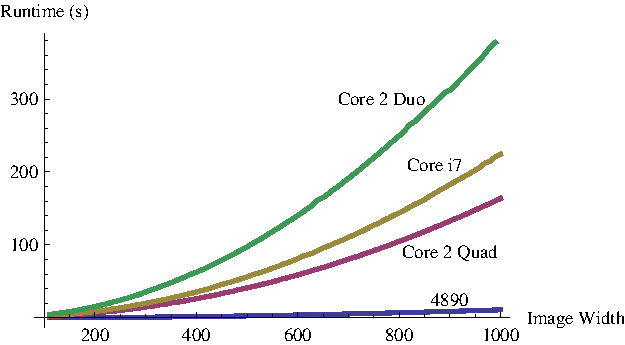
\includegraphics[width=84.5mm]{runtimePlot.pdf}
    \caption{Runtime vs. Resolution on All Hardware}
    \label{fig:runtimePlot}
\end{figure}

\begin{figure}
    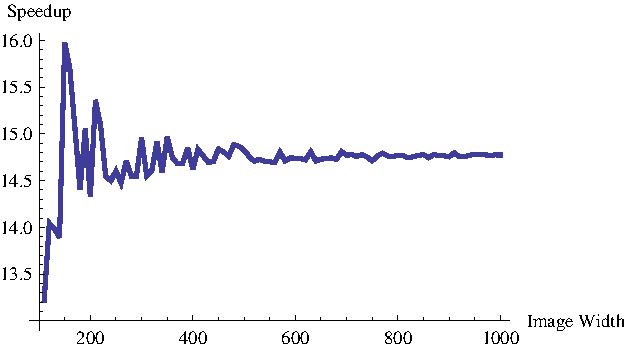
\includegraphics[width=84.5mm]{speedupPlot.pdf}
    \caption{Runtime vs. Resolution on All Hardware}
    \label{fig:runtimePlot}
\end{figure}

\subsection{Strong Scaling}

In order to measure the strong scalability of our implementation, we fix the problem size and vary the number of processing units used to compute it. For this benchmark, we will fix the image at $400\times400$ pixels, requiring $320,000,000$ total samples, and we will vary the number of cores of the 4890 that we use.

\begin{figure}
    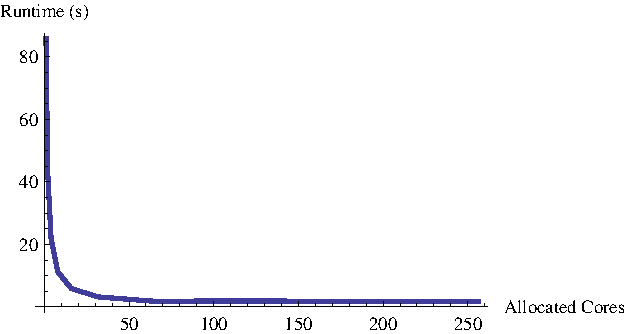
\includegraphics[width=84.5mm]{strongPlotOne.pdf}
    \caption{Core Count vs. Runtime on the 4890 with a fixed resolution ($400\times400$)}
    \label{fig:strongPlotOne}
\end{figure}

\begin{figure}
    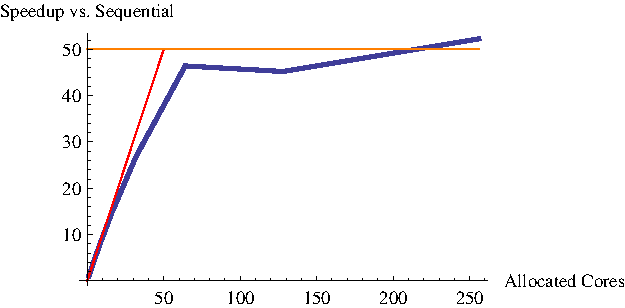
\includegraphics[width=84.5mm]{strongPlotTwo.pdf}
    \caption{Core Count vs. Speedup (measured against the single-core run) on the 4890 with a fixed resolution ($400\times400$); the orange line is the theoretical maximum speedup, given linear scaling and 50 execution units (800 cores / 16 cores per unit); the red line is a linear speedup curve}
    \label{fig:strongPlotTwo}
\end{figure}

One can see in figure \ref{fig:strongPlotTwo} that this implementation is strongly scalable; the speedup is almost perfectly linear as the core count increases. It should be noted that since the 4890 only has a maximum of 50 compute units, the linear increase is only maintained until we reach 50 cores; after that, the performance gains plateau as they should.

\subsection{Cost Effectiveness of Hardware}

\section{Future Work}

\section{Conclusion}

\section{Code}

All of the code developed for this project is available under the two-clause BSD license, and is hosted on GitHub:

\url{http://github.com/hortont424/orbitals}

\url{git://github.com/hortont424/orbitals.git}

The code has only been tested with the Apple and ATI OpenCL compilers, but should work with few to no changes on NVIDIA's SDK.

\bibliographystyle{acmsiggraph}
\nocite{*}
\bibliography{paper}

\end{document}